\section{Results}


\subsection{One and Two Body Unfolded Energy Terms}
\paragraph{}
We developed and implemented in Rosetta two energy terms which represent the one body and two body portions of the expected energy of a given residue type, called \textit{unfolded} and \textit{split\_unfolded\_two\_body} respectively. 
These terms constitute a two component reference energy, which can be used as a physical and statistical ``weight'' on a given residue type to bias design towards or away from sites of calculated low energy for that residue type.
These terms are extensible and can be applied to novel residue types, including peptidomemetics containing exotic backbone elements, with a minimum of additional development, and we present them here with all 20 canonical amino acids and a majority of Rosetta-implemented NCAA types functional.
The implementation of additional NCAA types that use only atom types listed in table \ref{tab:atypes_all} for use with these energy terms is intended to be a simple process, requiring only the generation of a one body low energy score set.
While the details of doing this differ slightly when additional backbone degrees of freedom are added, for residue types with rotation around only $\phi$ and $\psi$, an application is provided to generate these one body energies, found under \textit{src/apps/public/rileyse/FindMinEnergyOfDipeptideAA.cc} in the Rosetta code repository.
Usage details can be found in the methods section.

\paragraph{}
The \textit{unfolded} term we have implemented, while sharing much of it's code with the $unfolded$ score term implemented in 2012 Renfrew at al\cite{renfrew_incorporation_2012}, is distinct in function and generation from the older term.
The newer term consists of a sum of the intra-residue energy terms used in Rosetta for the residue in it's minimum energy dipeptide form(i.e. possessing capping acetyl and N-methyl groups to mimic adjacent backbone atoms), as a measure of the minimum energetic contribution of the residue to a folded protein structure.
The older term is an average energy of the residue when inserted as the central residue in a large number of five residue fragments from structured proteins, and includes two body energy terms as well, and is thus not directly comparable to this new \textit{unfolded} term.

\paragraph{}
The two body term \textit{split\_unfolded\_two\_body}, meanwhile, is an average intra-residue energy for a given residue type taken from many instances in folded protein structures from the top8000 high quality protein structure benchmark\cite{lovell_structure_2003}.
This term represents the expected two body energy of a residue in a folded protein context, and serves as a benchmark during design to tell how a designed instance of a residue type compares to the expected case, which is assumed to be a well satisfied instance of that residue type.


\subsection{Modifications to the mm\_std score function}
\paragraph{}
In addition to the development of our two component reference energy terms, we also made several revisions and updates to the \textit{mm\_std} score function, previously described by Renfrew et al in \cite{renfrew_incorporation_2012}, and which is currently the standard scoring function for non-canonical design tasks in Rosetta.
Since this score function was introduced, several significant updates to canonical protein scoring function were published with the introduction of the \textit{talaris2013} score function, which replaced \textit{score12\_full} as the standard Rosetta scoring function\cite{leaver-fay_chapter_2013}.
Some of these updates could be easily ported over to \textit{mm\_std}, specifically a proper electrostatics term, \textit{fa\_elec}, which was previously lacking in \textit{mm\_std}, and an updated disulfide bond term, \textit{dslf\_fa13}.
To adapt these terms, we adjusted the weights used in the \textit{talaris2013} score function relative to the difference in specific weights between the two score function.
In the case of \textit{fa\_elec}, we weighted it relative to the average of the hydrogen bonding score terms in \textit{mm\_std} versus those in \textit{talaris2013}, which were slightly higher in \textit{mm\_std}, resulting in a weight of 0.73 versus 0.70 for the \textit{fa\_elec} term in \textit{talaris2013}.
In the case of the \textit{dslf\_fa13} term, the old disulfide bond score terms in \textit{mm\_std} were identical to those from \textit{score12\_full}, and so the \textit{talaris2013} weight of 1.0 was used as-is.
The resulting score function weights file can be found in the Rosetta code repository as \textit{/database/scoring/weights/mm\_std\_fa\_elec\_dslf\_fa13.wts}.
To validate this improvement, we used the Rosetta sequence recovery benchmark, which showed much improved recovery of polar and charged residue types in the modified score function versus the original $mm\_std$.
The results of this test can be seen in table \ref{tab:performance}.
%Based on this result, we used this modified \textit{mm\_std} score function as the base for using our two component reference terms with \textit{mm\_std} in all further tests.


\subsection{Optimization of the one and two body term weights}
\paragraph{}
As the Rosetta score function is a composite of a diverse set of physical and statistical energy terms, adjusting the relative energetic contribution of each term via a set of score term weights is essential to achieve high performance on sequence recovery and other benchmark tasks\cite{rohl_protein_2004,leaver-fay_chapter_2013}.
As such, we fit weights $W_{2body}$ and $W_{1body}$ for \textit{unfolded} and \textit{split\_unfolded\_two\_body} respectively using the Rosetta sequence recovery benchmark test\cite{leaver-fay_chapter_2013} and a simple grid-based search technique.
We scanned combinations of $W_{2body}$ and $W_{1body}$ across the range of 1.0 to -1.0 for each weight(the typical range for Rosetta score term weights) in increments 0.1 for the \textit{talaris2013} score function, using the \textit{unique} atom type set.
The heat map of sequence recovery performance for this search can be found in figure \ref{fig:gridsearch_classes}.
Using the results of this scan to highlight the important regions of the weight space, we performed a series of higher resolution scans from -0.5 to 0.0 in increments of 0.05 using the elemental, mm and unique atom type sets for \textit{talaris2013}.
During early testing, we observed that the Rosetta/CHARMM atom types performed similar to but worse than the MM atom types, which are more specified.
As such, we excluded the Rosetta atom type set from the majority of our optimization and analysis process.
The results of these scans can be found in figures \ref{fig:gridsearch_atypes} and \ref{fig:gridsearch_classes}.
The top performing weight values for each combination of score function and atom type set among all scans were collected and can be found in table \ref{tab:performance}.
A longer ranged scan was also performed for \textit{talaris2013} with the unique atom type set, testing values between 5.0 and -5.0 in increments of 0.1, but the sequence recovery landscape beyond the 1.0 to -1.0 range was highly uniform, and thus was not explored further.

\subsection{Stability of sequence recovery results}
\paragraph{}
While the sequence recovery heat maps produced by our gridsearch process are both smooth and consistent across both score functions and atom type sets, we additionally confirmed the stability of the sequence recovery scores reported by computing 10 replicates sequence recovery tests using the best performing weight values from the \textit{talaris2013} unique atom type set grid search, shown below in table \ref{tab:performance}.
Using this set, we calculated a sample standard deviation of the replicates for each class of amino acid as well as the total. 
The standard deviation values obtained were 0.0094, 0.0202, 0.0274, and 0.0308 for hydrophobic, polar, positive, and negative amino acids respectively.
The standard deviation of the total sequence recovery was 0.0064.
The substantial decrease in standard deviation of the total compared to the individual classes suggests that while significant variance exists for most individual classes of amino acids, a decrease in one comes with a corresponding increase in another, and thus that total sequence recovery is largely of a zero sum process, wherein correct design of some positions prohibits correct design of others, and vice versa.
Given the similarity in shape of the performance space across the various configurations, we consider this test to be descriptive of the best performing weights of each configuration, particularly with respect to the total sequence recovery values reported.
%This is actually kind of an interesting late-breaking finding, the zero-sum-ness of design, at least for me. This stability question should probably be followed up on to look at per-amino-acid as well as mm\_std and baseline score functions without the split unfolded terms.

%Should probably make these grids bigger at some point...
\begin{figure}[hbtp]
  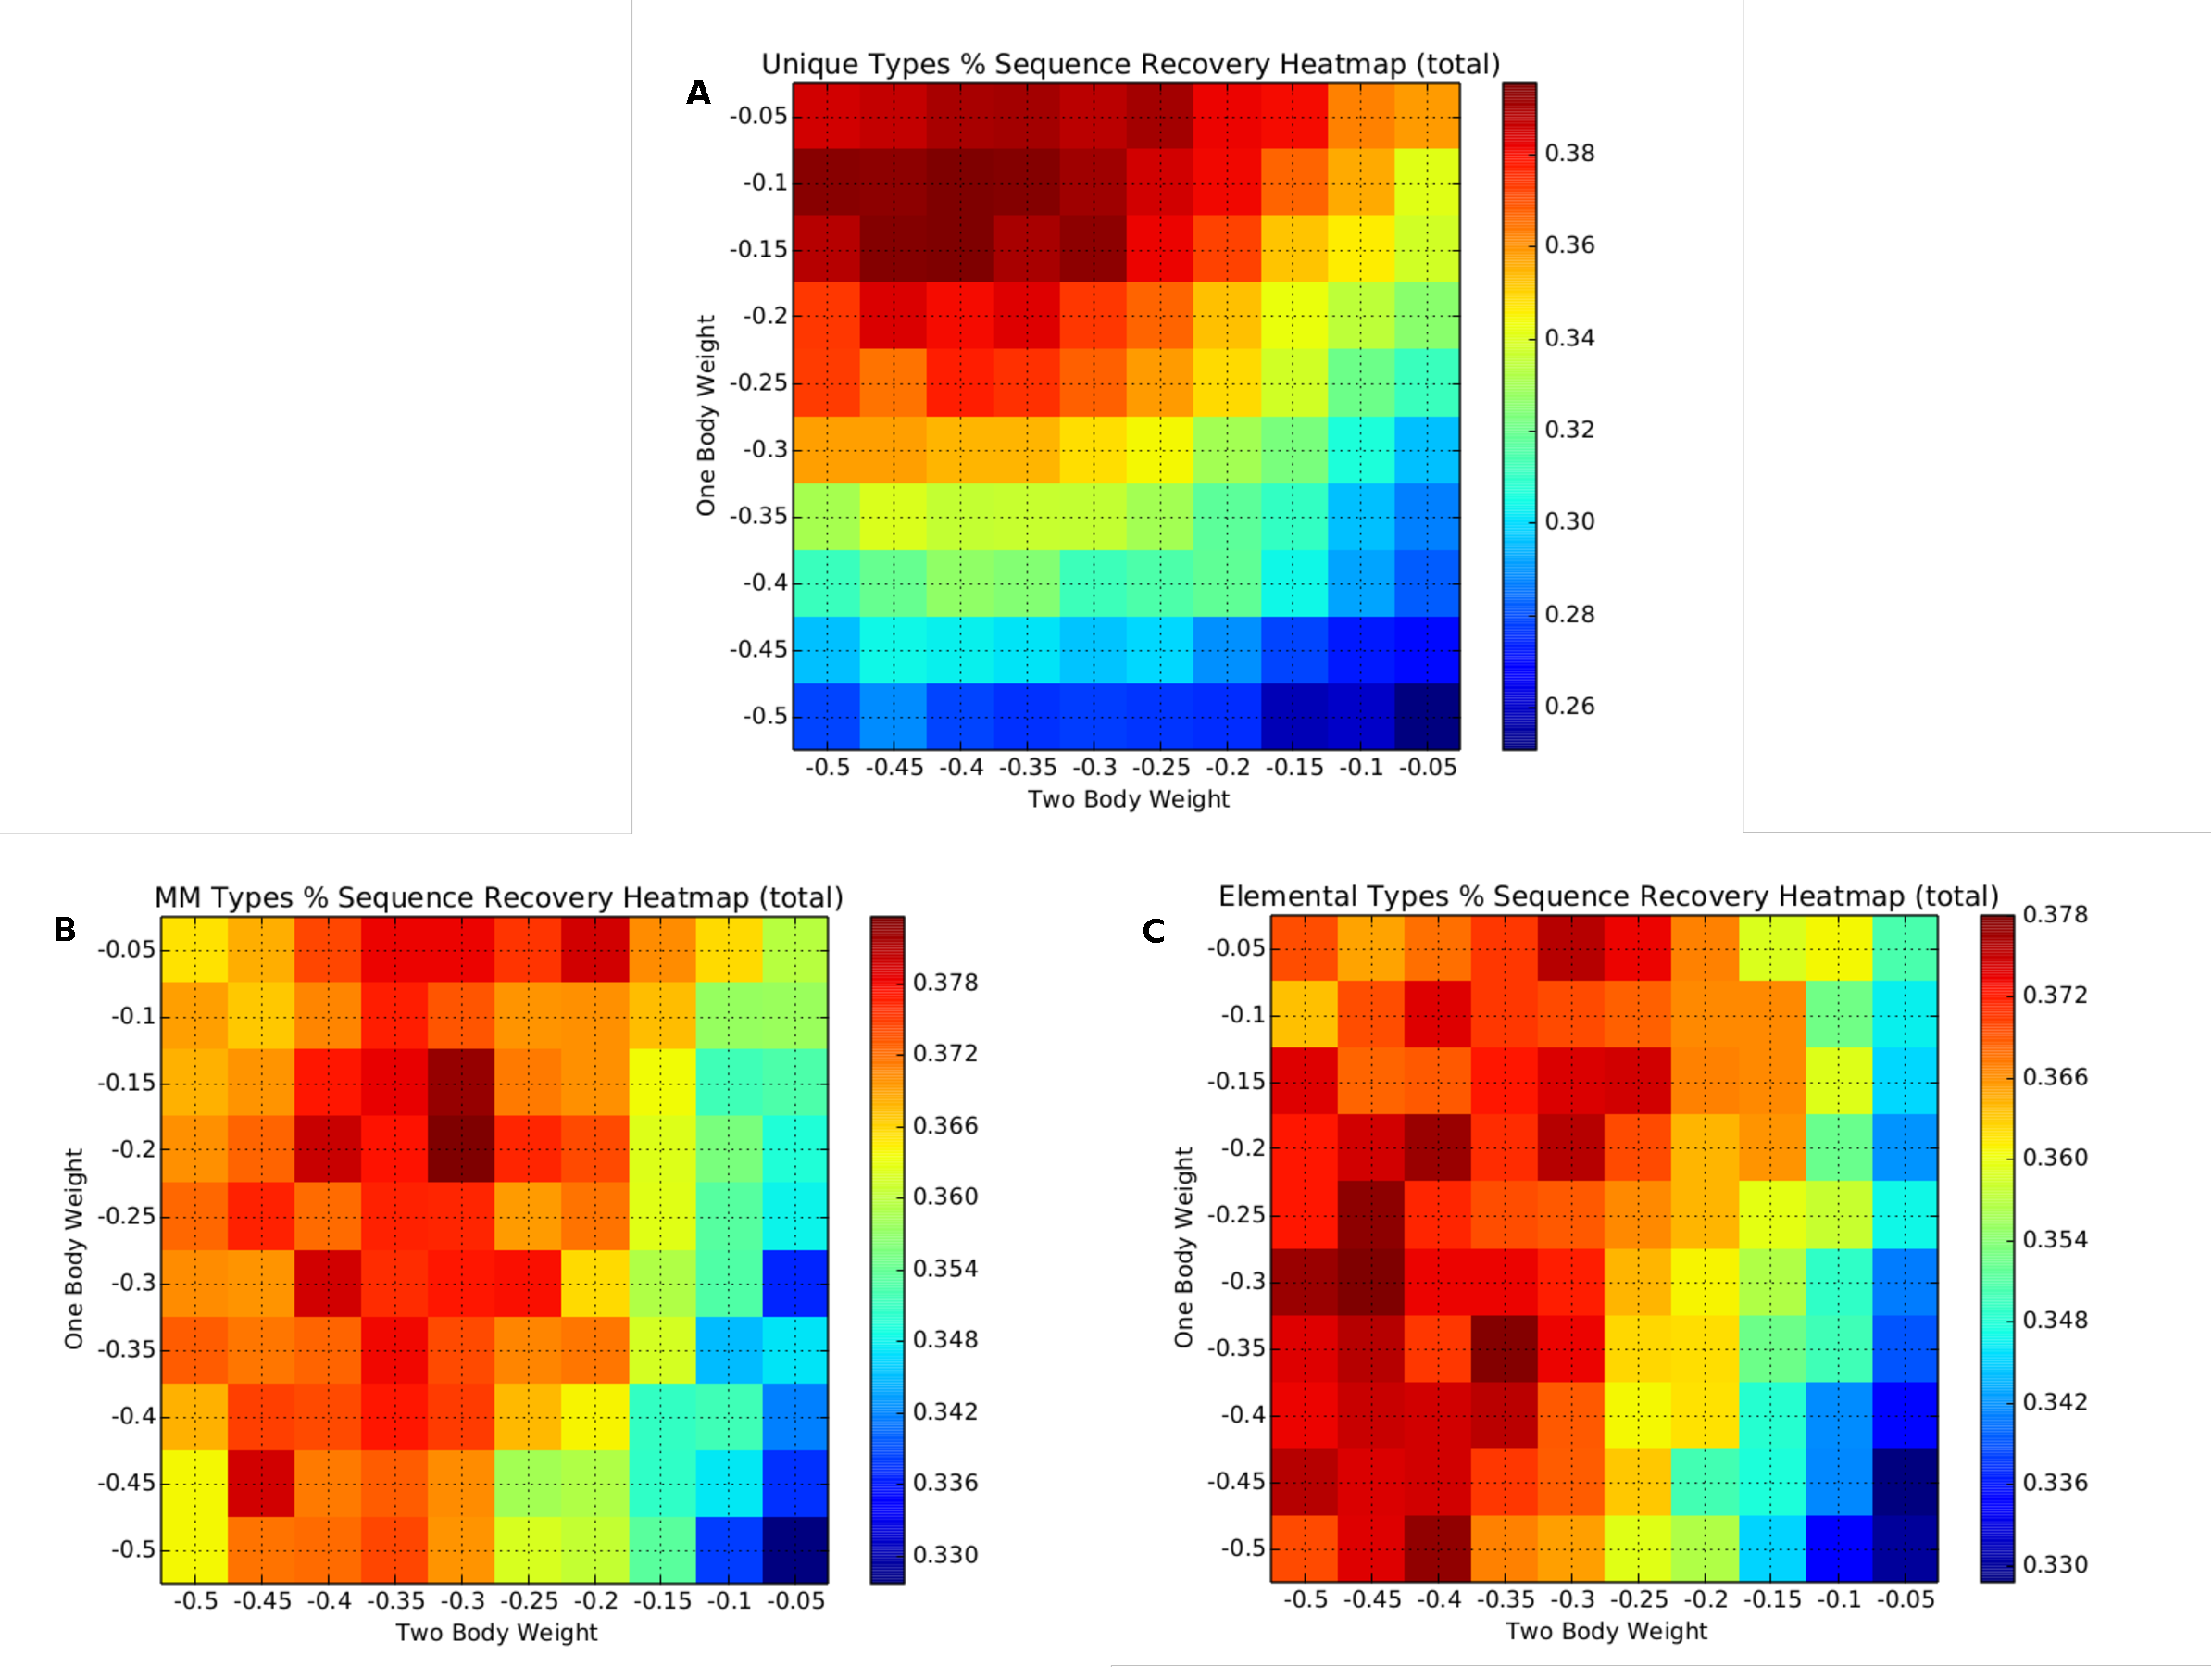
\includegraphics[width=\linewidth]{Figures/small_gridsearch_atom_type_sets.pdf}
  \caption{Heat maps showing total sequence recovery performance for \textit{talaris2013} using three different atom type sets for $W_{2body}$ and $W_{1body}$ values in the range of -0.5 to -0.05 in increments of 0.05.
  \textbf{A-C.} The total sequence recovery for the unique atom type set, the molecular mechanics atom type set, and the elemental atom type set respectively.}
  \label{fig:gridsearch_atypes}
\end{figure}


%This figure is actually outdated somewhat and should be regenerated when possible. Should still be broadly right, though.
\begin{figure}[hbtp]
  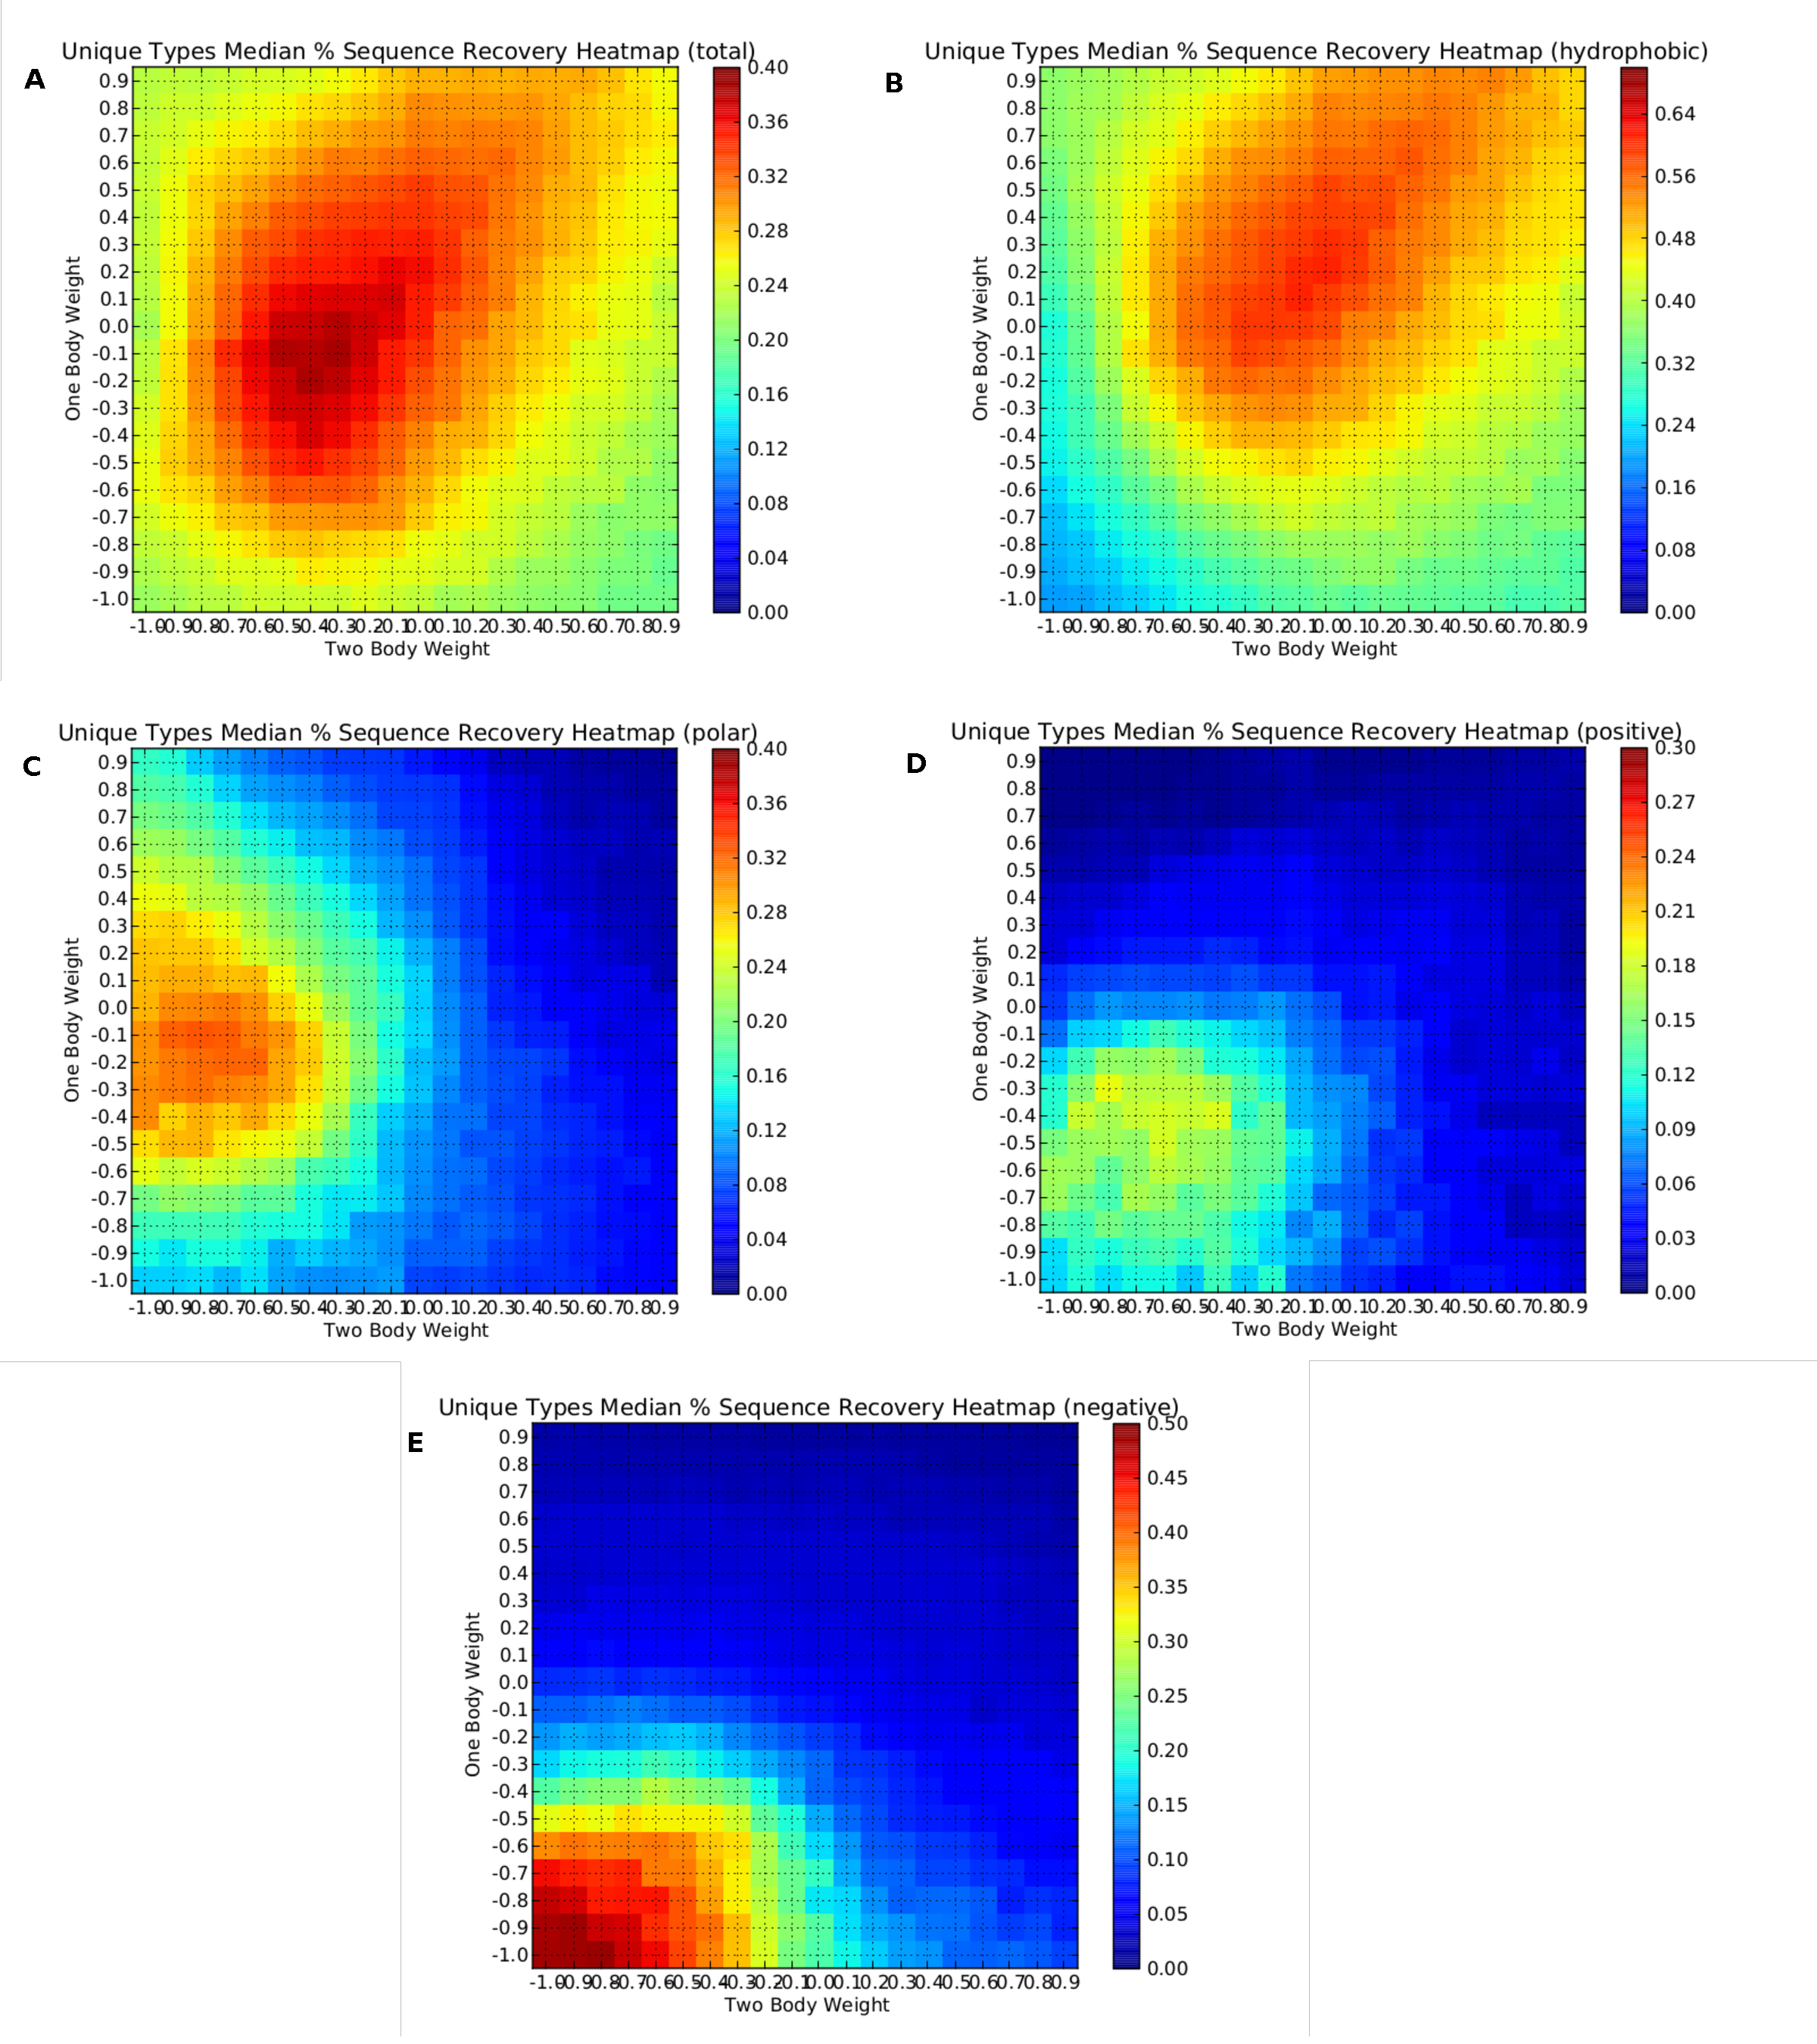
\includegraphics[width=\linewidth]{Figures/unique_types_broad_gridsearch_classes.pdf}
  \caption{Heat maps showing sequence recovery performance for \textit{talaris2013} using the unique atom type set for $W_{2body}$ and $W_{1body}$ values in the range of 1.0 to -1.0 in increments of 0.1.
  \textbf{A-E.} In order, the total sequence recovery, recovery for hydrophobic residues(VAL,ILE,LEU,MET,PHE,GLY,ALA,PRO,TRP,TYR), recovery for polar residues(SER,THR,ASN,GLN), recovery for positively charged residues(ARG,LYS,HIS), and recovery for negatively charged residues(ASP,GLU).}
  \label{fig:gridsearch_classes}
\end{figure}

\subsection{The two component reference energy is robust over diverse input energies}
\paragraph{}
Based on the results in figure \ref{fig:gridsearch_atypes}, we observe that the behavior of our two component reference energy terms in the explored weight space does change somewhat between the various two body atom sets, despite the scommon protocol for how the differing low level energetic inputs are combined.
Interestingly, however, the high recovery region of weight space for each atom type set seems to be mostly overlapping, though differing in shape somewhat, which suggests that the differences in weight space behavior are due to boundry behaviors rather than a major shift in the assembled reference energies of the amino acids.
Unexpectedly, we observe that the unique atom type set produces a much more defined high recovery plateau than either of the less-specified atom types, as well as having a much broader range of weight values within that plateau.

\paragraph{}
Further, we observe in table \ref{tab:performance} that sequence recovery with \textit{talaris2013} using elemental atom types(the most general lower bound on energetic specificity) is significantly higher than than that of \textit{talaris2013} with no reference energy term, suggesting that our two component energy terms are very robust to generalizations and imprecisions in their input energies.
In addition, that \textit{talaris2013} using unique atom types(the most specific upper bound on energetic specificity) performs best and the same with elemental types worst does suggest that the additional two body energy specificity of the unique atom type set, wherein each amino acid type is considered to have its own two body energy based only on atoms in that amino acid type, has significant benefits for sequence recovery.
%Note to self: Check out what the actual compiled reference values are for each amino acid at some point, and have a table of those.

%Table to illustrate the differences between the atom type sets. 
\begin{table}[!htbp]

\fontsize{9pt}{9pt}
\selectfont

\begin{tabular}{c|llllllll}
Score Function & AType Set & Total \% & Phobic \% & Polar \% & Pos \% & Neg \% & $W_{1body}$ & $W_{2body}$\\
\hline
\textbf{talaris2013} & \textbf{N/A} & \textbf{0.3935} & \textbf{0.5240} & \textbf{0.2410} & \textbf{0.1635} & \textbf{0.3155} & \textbf{N/A} & \textbf{N/A}\\
talaris2013(w/o $ref$) & N/A & 0.351 & 0.5816 & 0.1317 & 0.0616 & 0.0575 & N/A & N/A\\
talaris2013 & Elemental & 0.3780 & 0.6117 & 0.1692 & 0.0474 & 0.0933 & -0.3 & -0.45\\
talaris2013 & MM & 0.3836 & 0.6095 & 0.1811 & 0.0829 & 0.0933 & -0.2 & -0.3\\
\textbf{talaris2013} & \textbf{Unique} & \textbf{0.3955} & \textbf{0.5849} & \textbf{0.2335} & \textbf{0.1327} & \textbf{0.1448} & \textbf{-0.15} & \textbf{-0.4}\\
%Add mm_std stuff later, still waiting on runs to finish, mostly.
\hline
mm\_std(original) & N/A & 0.2484 & 0.4447 & 0.0180 & 0.0687 & 0.0 & N/A & N/A\\
mm\_std(new) & N/A & 0.2720 & 0.4374 & 0.0539 & 0.1185 & 0.0933 & N/A & N/A\\
%mm\_std(new w/o \textit{unfolded}) & N/A & 0.2009 & 0.3184 & 0.0180 & 0.1730 & 0.0437 & N/A & N/A\\

%more to come, eventually.
\end{tabular}

\fontsize{10pt}{11pt}
\selectfont
\caption{Performance on the Rosetta sequence recovery benchmark broken down by residue class for \textit{talaris2013}, \textit{mm\_std}, and \textit{mm\_std\_fa\_elec\_dslf\_fa13} score functions, plus variants using the two component reference energy terms and the stated two body atom type set.
Variant results shown are using the best discovered one and two body weights from the corresponding grid search.}
\label{tab:performance}

\end{table}


\subsection{The two component reference terms perform comparably to \textit{ref}}
\paragraph{}
Interestingly, while development of our two component reference energy was primarily motivated by the desire for compatability with NCAA's under the \textit{mm\_std} score function, it is surprisingly competitive with the statistical reference energy \textit{ref} under the \textit{talaris2013} score function.
Using the unique atom type set, our best set of weights achieved a level of sequence recovery comparable to that of \textit{talaris2013} with \textit{ref}---
We report in table \ref{tab:performance} a total sequence recovery of 0.3935 for \textit{talaris2013} using \textit{ref}, and a recovery of 0.3955 for \textit{talaris2013} using the two component reference terms, which are functionally equivalent given the level of variance described above.
In particular, we observe that the \textit{ref} reference energy's increase in sequence recovery over \textit{talaris2013} with no reference energy seems to derive mostly from increases in polar, positive, and negative amino acid recovery offset by a loss of hydrophobic recovery.
Meanwhile, \textit{talaris2013} with the two component reference energy displays a comparable level of hydrophobic performance to unreferenced \textit{talaris2013}, but manages to retain most of the polar amino acid recovery of \textit{ref} along with much of the positive and negative amino acid recovery.

%this is somewhat obsolete, as the composition of the one body term has changed slightly since then, and thus I would expect these numbers to be slightly better.
%Should probably also do another of these for mm_std as well at some point, though I'm not sure the code to generate it exists anymore(Doug had it).
%Also really needs some error bars...
\begin{figure}[hbtp]
  \includegraphics[width=0.65\linewidth]{Figures/aa_recovery_bar_plot_multi_line.png}
  \caption{Plot showing the percentage of all positions correctly designed for each residue type and each residue category.
Results for the standard \textit{talaris2013} scoring function are shown in green, \textit{talaris2013} without the \textit{ref} reference term in blue, and \textit{talaris2013} with \textit{ref} replaced by the two component reference terms.
The two body term was calculated using the unique atom type set, with weights of -0.15 and -0.4 for the one and two body terms respectively.}
  \label{fig:aa_recovery}
\end{figure}

\paragraph{}
The specific breakdown of sequence recovery by amino acid type can be found in figure \ref{fig:aa_recovery}, and shows that this trend is largely born out for each residue type.
Most two component reference energy amino acid recoveries are intermediate between the unreferenced \textit{talaris2013} recovery and that of \textit{talaris2013} plus \textit{ref}, though a few residue recoveries- specifically alanine, serine, threonine, histidine, and glycine- are higher than \textit{talaris2013} with or without \textit{ref} included.




%\subsection{$mm\_std$ sequence recovery is greatly increased by addition of the two component reference energy}
%hopefully, at least...

